\documentclass[11pt]{article}
\usepackage{amsmath,amssymb,amsthm}
\usepackage{url}
\usepackage{filecontents}
\usepackage{tikz}
\usepackage{xcolor, colortbl}
\definecolor{Gray}{gray}{0.9}


\DeclareMathOperator*{\E}{\mathbb{E}}
\let\Pr\relax
\DeclareMathOperator*{\Pr}{\mathbb{P}}

\newcommand{\handout}[5]{
  \noindent
  \begin{center}
  \framebox{
    \vbox{
      \hbox to 5.78in { {\bf CS 229r: Algorithms for Big Data } \hfill #2 }
      \vspace{4mm}
      \hbox to 5.78in { {\Large \hfill #5  \hfill} }
      \vspace{2mm}
      \hbox to 5.78in { {\em #3 \hfill #4} }
    }
  }
  \end{center}
  \vspace*{4mm}
}

\newcommand{\lecture}[4]{\handout{#1}{#2}{#3}{Scribes: #4}{Lecture #1}}

\newtheorem{theorem}{Theorem}
\newtheorem{corollary}[theorem]{Corollary}
\newtheorem{lemma}[theorem]{Lemma}
\newtheorem{observation}[theorem]{Observation}
\newtheorem{proposition}[theorem]{Proposition}
\newtheorem{definition}[theorem]{Definition}
\newtheorem{remark}[theorem]{Remark}
\newtheorem{claim}[theorem]{Claim}
\newtheorem{fact}[theorem]{Fact}
\newtheorem{assumption}[theorem]{Assumption}

% 1-inch margins, from fullpage.sty by H.Partl, Version 2, Dec. 15, 1988.
\topmargin 0pt
\advance \topmargin by -\headheight
\advance \topmargin by -\headsep
\textheight 8.9in
\oddsidemargin 0pt
\evensidemargin \oddsidemargin
\marginparwidth 0.5in
\textwidth 6.5in

\parindent 0in
\parskip 1.5ex

\begin{document}

\lecture{24 --- November 24, 2015}{Fall 2015}{Prof.\ Jelani Nelson}{Zhengyu Wang}

\section{Cache-oblivious Model}
Last time we talked about {\em disk access model} (as known as DAM, or {\em external memory model}). Our goal is to minimize I/Os, where we assume that the size of the disk is unbounded, while the memory is bounded and has size $M$. In particular, the memory is divided into $\frac{M}{B}$ pages, each of which is a block of size $B$. Today we are going to continue trying to minimize I/Os, but we are going to look at a new model called {\em cache-oblivious model} introduced in \cite{frigo1999cache} (you can also refer to the survey \cite{demaine2002cache} for more detail). The new model is similar to DAM, but with two differences (we further refer them as two assumptions):
\begin{enumerate}
\item Algorithms are not allowed to know $M$ or $B$. 
\item Algorithms do not control cache replacement policy. Operating system handles cache replacement, and we assume it makes optimal choices. (So in our analysis, we assume that we evict what we want to evict.)
 \end{enumerate}
Why do we have cache-oblivious model? First, it makes programs easily portable across different machines. You do not have to find parameters in your code for a specific machine. Note that the block size $B$ is chosen to amortize against the expensive cost of seeking on the disk. In really, $B$ is not fixed, because even on a given disk, there are multiple levels of memory hierarchy (L1/L2 cache, memory and disk), and we have different effective $B$'s to get the optimal amortized performance guarantee. Second,  your code might actually be running on a machine that are also running a lot of other processes at the same time. So the effective $M$ used by your process might change over time.  Therefore, our first assumption that we do not know $M$ or $B$ makes the model more robust. 

When first looking at the second assumption, it seems unrealistic to know optimal choices. In particular, the optimal choices depend on the future, because we should evict pages that would not be used in the near future. Actually, we can show that Assumption 2 is not a very idealized assumption, and it is fine to assume that the operation system knows about the future. The reason for that is related to some facts about online algorithms. In the following, we have a brief detour for online algorithms, in order to justify the optimal choices from the operating system.

Before doing the justification, let us make sure the model is not completely crazy. We actually have I/O efficient algorithms that do not know $M$ or $B$ beforehand. We have already seen one in the last lecture, which was scanning an array. Even if we do not know $B$, we can store elements in a continuous array. Then when you scan the array, the I/O complexity is $\frac{M}{B}$. So the bound depends on $B$, although the code does not know $B$. 

\subsection{Online Algorithms}

The idea of the online algorithms is, we have a sequence of events, and after each event we must make an irreversible decision.
One example of online problem is ski rental problem. Assume that you and your friends are on vacation. You do not have preference on how long the vacation is.  

\begin{itemize}
\item Every morning you wake up at the resort, you ask your friends if ``you want to continue skiing tomorrow'' or ``finish the vacation''. Your friends say ``continue skiing'' or ``we're done''.
\item In terms of expenses for skis, you have two options. The first option is to buy skis, which takes \$10 (no refunds). The second option is to rent skis, which takes \$1. 
\end{itemize}

On each day, if your friends decide to continue skiing, you need to decide whether buy skis or rent skis. Once you buy skis, in the future you do not need to pay extra expenses. The goal is to minimize cost ratio versus an omniscient being who knows future. The ratio is called ``competitive ratio''. Let $D=$\#days skiing, then $OPT=\min\{D,10\}$. If our strategy is to rent for the first $9$ days, and buy on $10$-th day, then we have worst case ratio $1.9$. 

If we are allowed to use randomness when making decisions, an expected competitive ratio of $\frac{e}{e-1}$ can be achieved\footnote{The result is covered in CS224 Fall 2014, \url{http://people.seas.harvard.edu/~minilek/cs224/lec/lec10.pdf}}. On the other hand, we have lower bound for deterministic algorithm, and a competitive ratio of $2-o(1)$ is the best possible (as the cost of buying skis goes to infinity).

\subsection{Paging Problem}

The problem is studied in \cite{sleator1985amortized}.
In the paging problem, the memory can hold $k=\frac{M}{B}$ pages,
and we have a sequence of page access requests. 
Just like the DAM model we have seen, if the page (a page is a block now) is in the memory, we can get access to it for free; 
if the page is not in the memory, we have to fetch it, bring it in, and evict some page in the memory (if the cost is $1$,
we get exactly the DAM model). 
In our situation, the online problem is choosing how to evict
memory. 
Again, we do not know the future. We have to decide which to evict on the fly. 
The omniscient algorithm would evict the page that will be
fetched again farthest in the future (in time). 
But we don't know the future, so what to do in the real
system? Two commonly used strategies/algorithms are:
\begin{description}
\item[LRU] (least recently used): for each page in the memory, keep track of when most recently I touched the page. And the page furthest back to the past is the one that we choose to evict. 
\item[FIFO] (first-in / first-out): we evict the oldest page in memory. 
\end{description}

These strategies are nice because of the following fact.

\begin{theorem}[Sleator-Tarjan \cite{sleator1985amortized}]
  \label{FIFOLRU}
  FIFO and LRU are:
  \begin{enumerate}
  \item $k$-competitive against $OPT$.
  \item $2$-competitive against $OPT$ when $OPT$ is given $k/2$
    memory.
  \end{enumerate}
\end{theorem}

Why does this justify the Assumption~2 of the cache-oblivious model? Well, as long as
$T(N,M,B) =\Theta(T(N,M/2,B))$, where $T(\cdot,\cdot,\cdot)$ is the cost given by
the analysis of our cache-oblivious algorithm, then Theorem~\ref{FIFOLRU} 
implies that using FIFO or LRU instead of the assumed
$OPT$ results in no (asymptotic) loss in performance.

\section{Some Cache-oblivious Algorithms}
Now we are going to look at some cache-oblivious algorithms\footnote{This section borrows largely from notes of CS229r Fall~2013 Lecture~22 scribed by Arpon Raksit.}.

\subsection{Array traversal/Reversal}

For traversal, as mentioned in the last lecture, the DAM algorithm
 is actually cache oblivious: we just scan the array in
blocks of size $B$ at a time. I/O cost is still at most $O(1+N/B)$.

For reversal, we can traverse the array backwards and forwards and
swap along the way. So by traversal cost, cost for reversal is
$O(1+N/B)$.

\subsection{Square Matrix Multiplication}

Here our DAM algorithm from last time does not carry over to the
cache-oblivious model, since we explicitly broke up the matrix into
sub-matrices of size $\sqrt{\frac{M}{2}}$ by $\sqrt{\frac{M}{2}}$. But we are still able to do
something simple. Note that we can choose how things layout in the memory. 
We recursively construct our layout. We first split our matrices into four blocks such that:
\[
\begin{pmatrix}
  A_{11} & A_{12} \\ A_{21} & A_{22}
\end{pmatrix}
\begin{pmatrix}
  B_{11} & B_{12} \\ B_{21} & B_{22}
\end{pmatrix}
=
\begin{pmatrix}
  A_{11}B_{11} + A_{12}B_{21} & A_{11}B_{12} + A_{12}B_{22}
  \\ A_{21}B_{11} + A_{22}B_{21} & A_{21}B_{12} + A_{22}B_{22}
\end{pmatrix},
\]
reducing multiplication of $N \times N$ matrices to eight
multiplications and four additions of $N/2 \times N/2$
matrices. Moreover, we will store our matrices $A$ and $B$ on disk as
follows.
\[
\begin{tabular}{|c|c|c|c|}
  \hline
  $A_{11}$ & $A_{12}$ & $A_{21}$ & $A_{22}$ \\
  \hline
\end{tabular}
\quad\quad
\begin{tabular}{|c|c|c|c|}
  \hline
  $B_{11}$ & $B_{12}$ & $B_{21}$ & $B_{22}$ \\
  \hline
\end{tabular}
\]
Then we apply this construction recursively (until the sub-matrix we want to store is $1\times 1$) for each $A_{ij}$ and
$B_{ij}$. For example, $A_{11}$ will be further decomposed (within the
decomposition of $A$ above) as follows.
\[
\begin{pmatrix}
  (A_{11})_{11} & (A_{11})_{12} \\ (A_{11})_{21} & (A_{11})_{22}
\end{pmatrix}
\quad\quad
\begin{tabular}{|c|c|c|c|}
  \hline $(A_{11})_{11}$ & $(A_{11})_{12}$ & $(A_{11})_{21}$ &
  $(A_{11})_{22}$ \\ \hline
\end{tabular}
\]
This gives us a recursive algorithm for matrix multiplication.

Let's analyze number $T(N)$ of I/Os. We have $8$ recursive multiplications,
and the additions just require scans over $O(N^2)$ entries. Thus
recurrence is given by $T(N) = 8\,T(\frac{N}{2}) + O(1+\frac{N^2}{B})$. The base
case is $T(\sqrt{M}) = O(\frac{M}{B})$ for $N\le\sqrt{M}$, since we can read an entire $\sqrt{M}
\times \sqrt{M}$ matrix into memory (due to the recursive data
layout!). Solving this gives $T(N) = O(\frac{N^2}{B} + \frac{N^3}{B\sqrt{M}})$.
For $N\ge M$, $\frac{N^3}{B\sqrt{M}}$ dominates $T(N)$, and we get $T(N)=O(\frac{N^3}{B\sqrt{M}})$.

\begin{remark}
  This technique of recursively laying out data to get locality, and
  then using $M$ and $B$ to get a good base case of our analysis, will
  be quite useful in many situations.
\end{remark}

\subsection{Linked Lists}

We want to support the following three operations: 
\begin{itemize}
\item Insert($x$, $p$): insert element $x$ after $p$;
\item Delete($p$): delete $p$;
\item Traverse($p$, $k$): traverse $k$ elements starting at $p$. 
\end{itemize}
\textbf{Shooting for:} $O(1)$ each insertion and deletion, and $O(1+k/B)$
to traverse $k$ elements (amortized).

\textbf{Data structure:} maintain an array where each element has pointers
to the next and previous locations that contain an element of the
list. But it will be self-organizing. 

\textbf{Insertion}($x$, $p$): append element $x$ to end of array. Adjust pointers accordingly. It costs $O(1)$ I/Os.

\textbf{Deletion}($p$): mark the array location specified by $p$ as deleted. It costs $O(1)$ I/Os.

But now elements might be far apart in the array, so on traversal
queries we're going to fix up the data structure (this is the
self-organising part).

\textbf{Traverse}($p$, $k$): we traverse as usual
using the pointers. But in addition, afterwards we delete the $k$
elements we traversed from their locations and append them to the end
of the array.

\[
\begin{tabular}{|p{5pt}|p{5pt}|p{5pt}|p{5pt}|p{5pt}|p{5pt}|p{5pt}|p{5pt}|p{5pt}|p{5pt}|p{5pt}|p{5pt}|p{5pt}|p{5pt}|p{5pt}|p{5pt}|p{5pt}|}
  \hline \cellcolor{Gray}4 & \cellcolor{Gray}1 & \cellcolor{Gray}2 & \cellcolor{Gray}3 &\cellcolor{Gray}
   \ \ & \cellcolor{Gray}5 & \cellcolor{Gray}\ \ & \cellcolor{Gray}6 & \cellcolor{Gray}\ \ & \cellcolor{Gray}\ \
   \cellcolor{Gray} &\ \ & \ \ & \ \ & \ \ & \ \ & \ \ & \\ \hline
\end{tabular}
\]
\vspace{3pt}
\[
\begin{tabular}{|p{5pt}|p{5pt}|p{5pt}|p{5pt}|p{5pt}|p{5pt}|p{5pt}|p{5pt}|p{5pt}|p{5pt}|p{5pt}|p{5pt}|p{5pt}|p{5pt}|p{5pt}|p{5pt}|p{5pt}|}
  \hline \cellcolor{Gray}X & \cellcolor{Gray}X & \cellcolor{Gray}X & \cellcolor{Gray}X & 
  \cellcolor{Gray}\ \ & \cellcolor{Gray}X & \cellcolor{Gray}\ \ & \cellcolor{Gray}X & \cellcolor{Gray}\ \ &
  \cellcolor{Gray}\ \ & \cellcolor{Gray}1 & \cellcolor{Gray}2 & \cellcolor{Gray}3 &
  \cellcolor{Gray} 4 &\cellcolor{Gray} 5 &\cellcolor{Gray} 6 & \\ \hline
\end{tabular}
\]

\textbf{Rebuild:} finally, after every $\frac{N}{2}$ operations (traverse counts as $k$ operations), 
rewrite entire data structure to a new contiguous array. Free the old one. 
This increases amortized complexity of each operation by $O(\frac{1}{B})$. 

Now, what does traversal cost? When we do a traversal, we touch $r$
contiguous runs of elements. Thus the number of I/Os in the traversal
is $O(r + k/B)$------one I/O for each run, and the cost of a scan of the $k$
elements. But there must have been $r$ updates to cause the gaps
before each run. We amortize the $O(r)$ over these $r$ updates, so
that traversal costs $O(k/B)$ amortized. (To be more precise: any
sequence of $a$ insertions, $b$ deletions, and a total of $k$ items
traversed costs $O(a + b + 1 + k/B)$ total I/Os.) And since after a
traversal we consolidate all of the runs, the $r$ updates we charged
here won't be charged again.

\begin{quote}
  ``One money for me means one I/O.'' -- Jelani Nelson
\end{quote}

That's amortized linked lists. See \cite{bender2002two} for worst-case data structure.

\subsection{Static $B$-tree}

We're going to build a $B$-tree (sort of) without knowing $B$. The
data structure will only support queries, that is, no insertions
\cite{frigo1999cache}. For dynamic B-tree, refer to \cite{bender2005cache}. We will use another recursive layout strategy,
except with binary trees. It looks as follows (conceptual layout on
left, disk layout on right). Keep in mind this picture is recursive
again.

\[
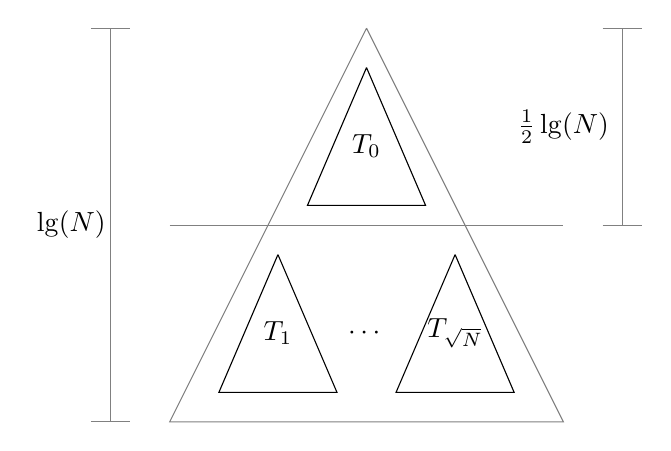
\begin{tikzpicture}[scale = 2.5, baseline=70pt]
  \draw[gray] (1,2) -- (0,0) -- (2,0) -- (1,2);
  \draw (1,1.8) -- (0.7,1.1) -- (1.3,1.1) -- (1,1.8);
  \draw (0.55,0.85) -- (0.25,0.15) -- (0.85,0.15) -- (0.55,0.85);
  \draw (1.45,0.85) -- (1.15,0.15) -- (1.75,0.15) -- (1.45,0.85);

  \draw (1,1.4) node {$T_0$};
  \draw (.55,.45) node {$T_1$};
  \draw (1.45,.45) node {$T_{\sqrt{N}}$};
  \draw (1,.45) node {$\cdots$};

  \draw[gray] (0,1) -- (2,1);

  \draw[gray] (-.3,0) -- (-.3,2);
  \draw[gray] (-.4,0) -- (-.2,0);
  \draw[gray] (-.4,2) -- (-.2,2);
  \draw (-.5,1) node {$\lg(N)$};

  \draw[gray] (2.3,1) -- (2.3,2);
  \draw[gray] (2.2,1) -- (2.4,1);
  \draw[gray] (2.2,2) -- (2.4,2);
  \draw (2.0,1.5) node {$\frac{1}{2}\lg(N)$};
\end{tikzpicture}
\hspace{50pt}
\begin{tabular}{|c|c|c|c|}
  \hline $T_0$ & $T_1$ & $\cdots$ & $T_{\sqrt{N}}$ \\ \hline
\end{tabular}
\]

We query as usual on a binary search tree. To analyse the I/O cost,
consider the first scale of recursion when the subtrees/triangles have
at most $B$ elements. Reading in any such triangle is $O(1)$ I/Os. But
of course there are at least $\sqrt{B}$ elements in the tree, so in
the end traversal from root to leaf costs $O(2\cdot \log(N)/\log(\sqrt{B})) =
O(\log_B N)$ I/Os.

\subsection{Lazy Funnel Sort}

Original funnel sort is due to \cite{frigo1999cache}, simplified by
\cite{brodal2002cache}. Yet another recusrive layout strategy, but a
lot funkier. Assume we have the following data structure.

\begin{definition}
  A \emph{$K$-funnel} is an object which uses $O(K^2)$ space and can
  merge $K$ sorted lists of total size $K^3$ with $O((K^3/B)
  \log_{M/B}(K^3/B) + K)$ I/Os.
\end{definition}

Lazy funnel sort splits the input into blocks of size $N^{2/3}$,
recuseively sorts each block, and merges blocks using the $K$-funnel,
with $K = N^{1/3}$.
\[
\begin{tabular}{|c|c|c|c|}
    \hline $N^{2/3}$ & $N^{2/3}$ & $\cdots$ & $N^{2/3}$ \\ \hline
  \end{tabular}
\]

When analysing this, we will make the following \emph{tall cache
  assumption}. Unfortunately this assumption is required to get the
desired $O((N/B) \log_{M/B}(N/B))$ I/Os for sorting
\cite{brodal2002cache}.

\begin{assumption}[Tall cache]
  Assume $M = \Omega(B^2)$. But note that this can be relaxed to $M =
  \Omega(B^{1+\gamma})$ for any $\gamma > 0$.
\end{assumption}

We're running low on time so let's just see what the $K$ funnel
is. It's another recursive, built out of $\sqrt{K}$-funnels. The
funnels are essentially binary trees, except with buffers (the
rectangles, with labelled sizes) attached.

%% Please also excuse this nonsense.
\[
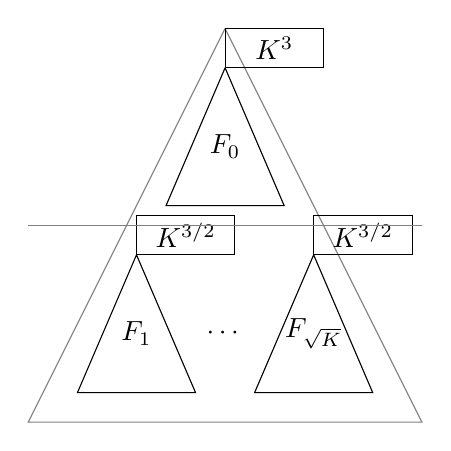
\begin{tikzpicture}[scale = 2.5, baseline=70pt]
  \draw[gray] (1,2) -- (0,0) -- (2,0) -- (1,2);
  \draw (1,1.8) -- (0.7,1.1) -- (1.3,1.1) -- (1,1.8);
  \draw (0.55,0.85) -- (0.25,0.15) -- (0.85,0.15) -- (0.55,0.85);
  \draw (1.45,0.85) -- (1.15,0.15) -- (1.75,0.15) -- (1.45,0.85);

  \draw (1,1.4) node {$F_0$};
  \draw (.55,.45) node {$F_1$};
  \draw (1.45,.45) node {$F_{\sqrt{K}}$};
  \draw (1,.45) node {$\cdots$};

  \draw (1.0,1.8) rectangle (1.5, 2.0);
  \draw (0.55,0.85) rectangle (1.05, 1.05);
  \draw (1.45,0.85) rectangle (1.95, 1.05);

  \draw (1.25,1.9) node {$K^3$};
  \draw (0.8,.95) node {$K^{3/2}$};
  \draw (1.7,.95) node {$K^{3/2}$};

  \draw[gray] (0,1) -- (2,1);
\end{tikzpicture}
\hspace{50pt}
\begin{tabular}{|c|c|c|c|c|}
  \hline $F_0$ & buffers & $F_1$ & $\cdots$ & $F_{\sqrt{K}}$ \\ \hline
\end{tabular}
\]

At each level the $\sqrt{K}$ buffers use $O(K^2)$ space. Then the
total space used is given by the recurrence $S(K) =
(1+\sqrt{K})S(\sqrt{K}) + S(K^2)$. Solving this gives $S(K) \le
O(K^2)$.

How do you use a $K$-funnel to merge? Every edge has some buffer on
it (which all start off empty). The root node tries to merge the contents of the buffers of the two edges to its children. If they are empty, the root recursively asks its children to fill their buffers, then proceeds to merge them. The recursion can go all the way down to the leaves, which are either connected to the original $K$ lists to be merged, or are connected to the output buffers of other funnels created at the same level of recursion (in which case you recursively ask them to fill their output buffers before merging). 

\begin{theorem}
  As described, lazy funnel sort costs $O((N/B) \log_{M/B}(N/B))$ I/Os
  (under the tall cache assumption).
\end{theorem}

\begin{proof}[Proof sketch]
  The recurrence above proved funnel property (1). For funnel property
  (2), look at the coarsest scale of recursion where we have $J$
  funnels, with $J \ll \sqrt{M}$. The details are in
  \cite{demaine2002cache}.
\end{proof}


 
\newpage
\begin{filecontents}{shortbib.bib}
@incollection{bender2002two,
  title={Two simplified algorithms for maintaining order in a list},
  author={Bender, Michael A and Cole, Richard and Demaine, Erik D and Farach-Colton, Martin and Zito, Jack},
  booktitle={Algorithms?ESA 2002},
  pages={152--164},
  year={2002},
  publisher={Springer}
}
@inproceedings{brodal2002cache,
  title={Cache oblivious search trees via binary trees of small height},
  author={Brodal, Gerth St{\o}lting and Fagerberg, Rolf and Jacob, Riko},
  booktitle={Proceedings of the thirteenth annual ACM-SIAM symposium on Discrete algorithms},
  pages={39--48},
  year={2002},
  organization={Society for Industrial and Applied Mathematics}
}
@article{demaine2002cache,
  title={Cache-oblivious algorithms and data structures},
  author={Demaine, Erik D},
  journal={Lecture Notes from the EEF Summer School on Massive Data Sets},
  volume={8},
  number={4},
  pages={1--249},
  year={2002}
}
@inproceedings{frigo1999cache,
  title={Cache-oblivious algorithms},
  author={Frigo, Matteo and Leiserson, Charles E and Prokop, Harald and Ramachandran, Sridhar},
  booktitle={Foundations of Computer Science, 1999. 40th Annual Symposium on},
  pages={285--297},
  year={1999},
  organization={IEEE}
}
@article{sleator1985amortized,
  title={Amortized efficiency of list update and paging rules},
  author={Sleator, Daniel D and Tarjan, Robert E},
  journal={Communications of the ACM},
  volume={28},
  number={2},
  pages={202--208},
  year={1985},
  publisher={ACM}
}
@article{bender2005cache,
  title={Cache-oblivious B-trees},
  author={Bender, Michael A and Demaine, Erik D and Farach-Colton, Martin},
  journal={SIAM Journal on Computing},
  volume={35},
  number={2},
  pages={341--358},
  year={2005},
  publisher={SIAM}
}
}
\end{filecontents}
\bibliographystyle{alpha}
\bibliography{shortbib}
\end{document}
